%%%--------------------------------%%%
%%% Implementation
%%%--------------------------------%%%

\section{Risk Use Cases}
\label{sec:implementationRisks}

Due to the interconnection between most of the risk use cases, they will be demonstrated by one larger example. First of all, the Risk CRUD (\ref{sec:domainBbd}) which includes the creation and editing of a risk: When opening the detail view of a project, the user will be able to propose a risk by providing a title and a more detailed description. After proposing, every project member has the chance to like this proposed risk and after reaching a specific amount of likes, the risk will then be discussable. All of this is additionally part of the Risk Discussion use case (\ref{sec:domainBbg}). This is intentionally missing the ability to provide negative textual feedback as the application cannot and is not supposed to substitute the discussion process between users. It is meant to be a facilitation of meetings but personal discussion is still important and necessary. The implementation of both use cases had a very high priority as the existence of risks, including their status change, is essential for the applications purpose. It is furthermore the direct foundation of use cases which require the existence of risks like the Risk Monitoring (\ref{sec:domainBbh}) or the Risk Pool (\ref{sec:domainBbf}). Figure \ref{fig:ShotProjectCreation} shows a proposed risk with two likes.

\begin{figure}[H]
	\centering
	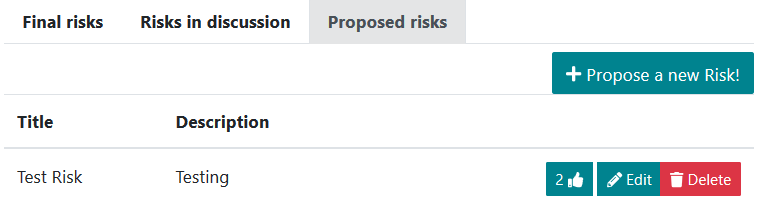
\includegraphics[width=0.6\textwidth]{Assets/implementation_shots/proposed_risk.png}
	\caption{Screenshot of a proposed risk with two supporters}
	\label{fig:proposedrisk}
\end{figure}

As the next step in the discussion process the risk will then be displayed beneath the "Discuss" tab within the project view. From here users are able to provide an estimation of risk severity and probability as seen in figure \ref{fig:riskdiscussion}.

\begin{figure}[H]
	\centering
	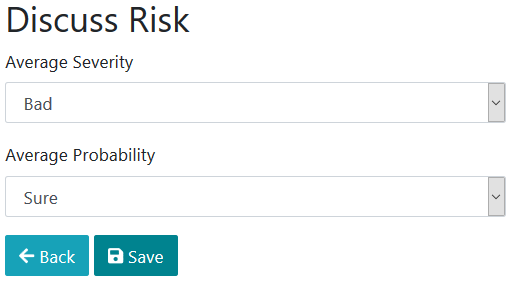
\includegraphics[width=0.6\textwidth]{Assets/implementation_shots/riskdiscussion.png}
	\caption{Screenshot of risk discussion}
	\label{fig:riskdiscussion}
\end{figure}

After enough estimations have been provided, a median estimation will be calculated and the project risk is ready to be finalized. In this step, one user has to assign themselves as owner of the risks, for which gamification rewards will be gained (\ref{sec:implementationRisks}), and multiple responses have to be defined. The latter is part of the Risk Response Management use case (\ref{sec:domainBbi}). If the above mentioned steps have been fulfilled, the risk will be final and then be displayed beneath the "Final" tab which opens automatically when opening the detailed project view.

 Missing from the MVP, is the ability to monitor risks with the help of notifications and a due date as described in the corresponding use case (\ref{sec:domainBbh}). This feature was omitted in favor of gamification use cases as it is not one of the necessary core functions of the risk management. However notifications themselves are already realized and due to the general design of the messaging functionalities the groundwork for this use case is present and it is ready to be realized in potential future iterations.
 
\begin{wrapfigure}{r}{0.5\textwidth}
	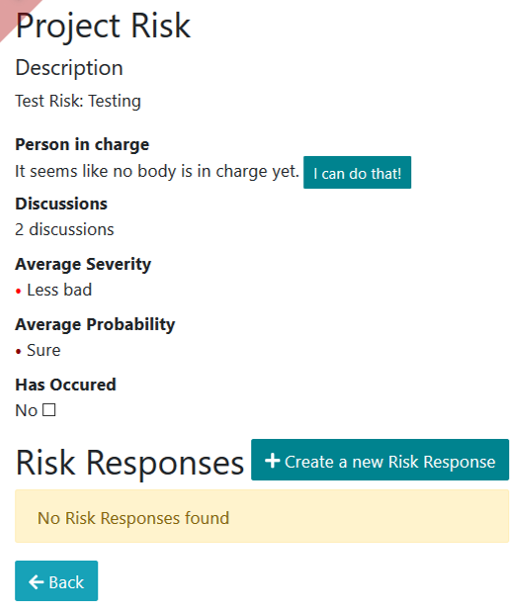
\includegraphics[width=0.5\textwidth]{Assets/implementation_shots/riskfinalization.png}
	\caption{Screenshot of finalization step}
	\label{fig:riskdfinalization}
\end{wrapfigure}

 Adjusting risk prioritization is also not possible yet but could be implemented like use case Project Risk Adjustment depicts (\ref{sec:domainBbe}). This use case aims at detail adjustment for the already implemented discussion use case and is therefore not a core feature.\\
 Also not part of the MVP is the Risk Pool (\ref{sec:domainBbf}). Despite being defined as criterion in the theory section (\ref{sec:theoryAd}) and being of specific interest for one of our reviewing PMs  (\ref{sec:DomainAb}) we decided to not integrate this use case. The Risk Pool is particularly valuable for coordination and learning processes across a company. The next testing and feedback loops however are rather unlikely to be of such a scope which is why features than can be evaluated by individual testers or teams where prioritzed for the \ac{MVP}.
 
 To conclude, Risk- and Risk Response Management are functionally implemented, as well as Risk Discussion. These features cover the basic project risk management functions necessary for a single project to be managed using the application sufficiently for an \ac{MVP}.
 